%!TEX root = ../dissertation.tex

\chapter{DMNApp: An Android Application}

\newthought{To evaluate the model on the wild}, and to provide some perspectives on the real-world applications of this problem, a frontend client for this task is proposed. As most image-based applications, it is necessary to acknowledge and recognize some of the design requirements involved in the implementation of such programs. In this case, for testing and evaluation purposes it has been decided to target a mobile application as final device frontend, as it allows the final users to test the DMN characteristics in-place, without having to upload an stored image onto a different web platform. Also, it is desired that the final application does integrate with native hardware devices, such as the device integrated camera(s), the microphone and additionally, access to the native localization services provided via GPS/GLONASS/GALILEO or via IP.

The main motivation behind this development consists in providing the building blocks necessary to design and build mobile applications that can be used to test computer vision models on the wild, as a generic proof-of-concept backend framework to provide Computer Vision services is proposed. On the present example and more specifically to this application, we use these set of building blocks to generate a visualization application for segmentation models, and more specifically, for language-based image segmentation tasks. It is necessary to add that this aplication can be extended to sort and categoriize images by more strong natural language criterions, instead of using object tags as most current applications do, it is possible to filter images based on a object referral expression, however, due to time constraints, this application is out of the scope of the present implementation.

On Figure~\ref{Fig:App_Overview}, a summary of the general overview of the application is presented, describing the interaction between different device hardware/software elements, such as the camera/gallery to adquire an image and the microphone/keyboard to get a query phrase that is going to be processed by the DMN. As a result, the user can visualize and threshold the final segmentation using different values, the visualization can be customized by choosing different mask colors or by displaying the final result as a heatmap on different colormaps. Finally, the user can export a result to an image or share it with another application installed.

\begin{figure}
    \centering
    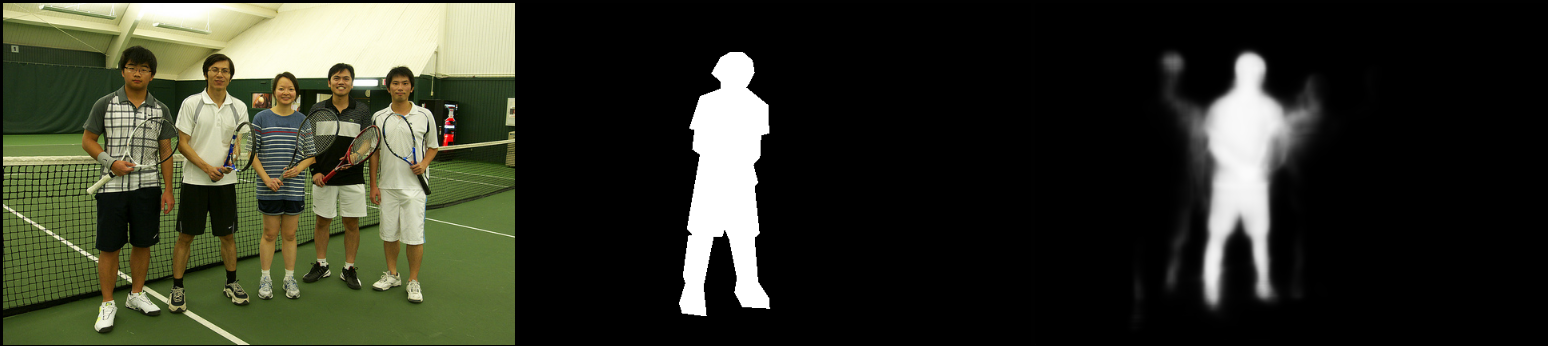
\includegraphics[width=\textwidth]{./figures/unc_samples/3.png}
    \caption{DMNApp general overview}
    \label{Fig:App_Overview}
\end{figure}